\section{Test Strategy}
For our project an Incremental Testing approach is used. The reason for this is that in Incremental Testing we use a combination of Bottom-Up and Top-Down Testing. This is a good approach because, in Scrum, the most critical Backlog Items will always be chosen first. Scrum testing is a very iterative process, and all User Stories shall be tested in one way or another.\\
\\
At the end of all Sprints we should be able to deliver a Potentially Shippable Product Increment based on the Sprint Backlog. This is significant for the model, because when work is divided into simple pieces it can be finished in a short period of time. Before we can address a part of our system as a Potentially Shippable Product Increment each User Story from the Sprint Backlog needs to be tested. To be able to verify a User Story, we determine specific Acceptance Criteria. These are formulated based on the Agile GIVEN, WHEN and THEN-method, also called Gherkin. This method makes it easy to test small parts of the system. The tests done based on the Acceptance Criteria are often called Unit Tests.\\
\\
There will be performed a set of verification tests in each Sprint relating to the User Story as mentioned above. Verification tests helps us verify that we have developed the right solution based on the Acceptance Criteria stated \cite{ref1}. Verification tests helps us determine if we are building the product right. In addition to this, the system also needs to be validated. With validation tests we make sure that we build the right product \cite{ref5}. In the case of building a Variable Pitch Quadrotor and comparing its attributes with a Fixed Pitch Quadrotor, the validation of our product will be the knowledge gained and a presentation when these are compared. \\
\\
\newpage

\subsection{Gherkin Syntax}
As mentioned earlier we use Gherkin Syntax to formulate our Acceptance Criteria. This is a good approach to write a human-readable story that describe a wanted behavior, which makes testing easier \cite{ref7}. This approach is often used in software development and testing, but for our project this gives us an easy description of a wanted behaviour for all parts of our system. In Tab. \ref{tab:gherkin} the syntax adopted is explained. 
\begin {table}[h]
    \begin{center}
    \caption {Gherkin Syntax} 
    \label{tab:gherkin} 
    \begin{tabular}{|l|l|}\hline 
    GIVEN   &   Some Precondition \\ \rowcolor{gainsboro}
    AND    &   Some Other Precondition        \\
    WHEN    &   Some Action        \\ \rowcolor{gainsboro}
    AND    &   Yet Another Action        \\
    THEN    &   Some Testable Outcome is Achieved       \\ \rowcolor{gainsboro}
    AND    &   Something else we can Test Happens too.   \\
    \hline
    \end{tabular}
    \end{center}
\end{table}
\\
Out of this syntax we get a Test Case with a testable Acceptance Criteria. An Acceptance Criterion relates back to the User Story, the User Story relates back a Product Backlog Item, and the Product Backlog Item relates back to a need of the customer.Test methods will be chosen based on what we are testing.\\
\\
In Fig. \ref{fig:ACmatrix} our Acceptance Criteria for Sprint 1 are displayed. They were generated using Gherken Syntax.

\begin{figure}[h]
    \centering
        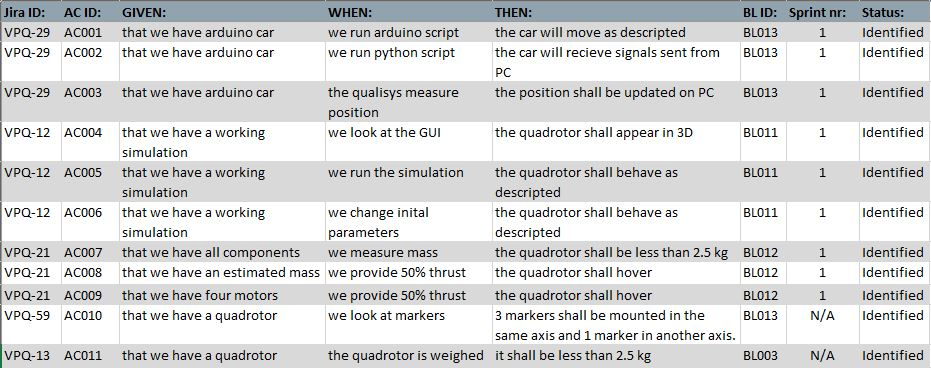
\includegraphics[width=1\textwidth]{VAPIQ-PICTURES/Capture2}
        \caption{Acceptance Criteria Tractability Matrix}
        \label{fig:ACmatrix}
\end{figure}


\newpage

\subsection {Test Setup}
The template presented below functions as a Verification record where our Acceptance Criterion is tested. This represents the Test Case where each card states an unique test ID. The Test Case displays which Acceptance Criteria, Backlog Item and Jira ID it relates to and in which Sprint the verification of Acceptance Criteria has been done. It also displays which Verification Procedure used and the results of the tests. The Test Case has been given an ID in the form of TXXX, where the XXX will be numbers. Each Test Cases will be numbered chronologically as we progress in the project. \\
\\
\testcard{TXXX}{ACXXX}{X}{BLXXX}{VPQ-XX}
         {\shortstack[l]{GIVEN, WHEN, THEN}}
         {\shortstack[l]{}}
         {\shortstack[l]{TRXXX}}
         {\shortstack[l]{}}

\subsubsection{Verification Procedure}
In the Verification Procedure row shown above, we will state which Test Method we have used and what order or in which steps the test shall be conducted. These procedures will be generated for every Test Case in every Sprint. Sometimes a Static Testing approach will be implemented and other times a Dynamic. We will also state in the Verification Procedure if special Test Equipment is needed to perform the tests.
\\
\subsubsection{Results and Reports}
Many Test Cases are easily executed because of the Gherkin Syntax, but some tests are more extensive and demands a more detailed procedure. The verification process sometimes need more elaboration. In these situations a Test Report is generated. The Test Report generated will be referred to in the Result(s)/Report(s) row as shown in the template above. The Test Report has been given an ID in the form of TRXXX, where the XXX will be numbers. Each Test Report will be numbered chronologically as we progress in the project. \\ 
\\
The test results are crucial to be able to verify our system. The test results gives us feedback if something is or is not functioning as the Acceptance Criteria specifies. Continuous testing of every criterion will help us with the verification of our system. This will again help us validate that we have come up with the right end result.\\
\newpage

\subsection{Test Traceability Matrix}
In Fig. \ref{fig:matrix} a matrix for Test Cases and relating Acceptance Criteria for Sprint 1 are displayed.

\begin{figure}[h]
    \centering
        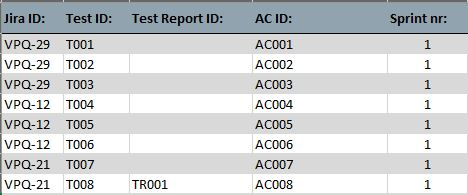
\includegraphics[width=0.9\textwidth]{VAPIQ-PICTURES/Capture}
        \caption{Test Taceability Matrix}
        \label{fig:matrix}
\end{figure}

\newpage

\subsection{Test Processes}
In Fig. \ref{fig:testsetup} we see a simple illustration of how our Verification Test process works for one Product Backlog Item. The Test Cases and Test Reports will include all the information needed for verification of our system and this will be found in the Test Specification Document.\\
\\
\begin{figure}[h]
    \centering
        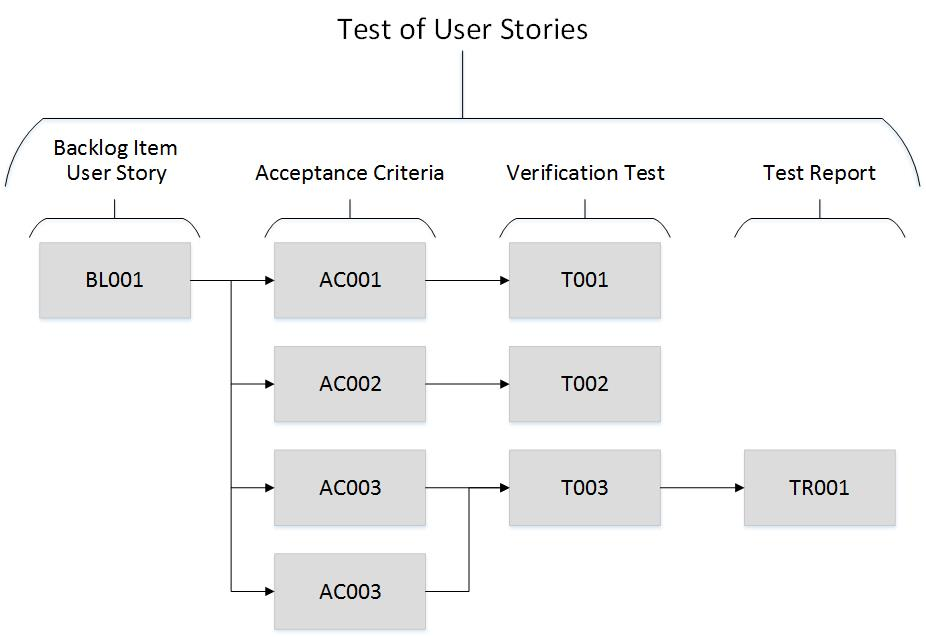
\includegraphics[width=0.8\textwidth]{VAPIQ-PICTURES/testdocbild}
        \caption{Test of Backlog Item}
        \label{fig:testsetup}
\end{figure}
\\
Fig. \ref{fig:testsetup} shows only an example of how we will test User Stories. This figure is not related to any already performed tests.\\

\newpage
In Fig. \ref{fig:testsetup2} we see a simple illustration of how our Verification Test Process works for one Sprint Backlog.

\begin{figure}[h]
    \centering
        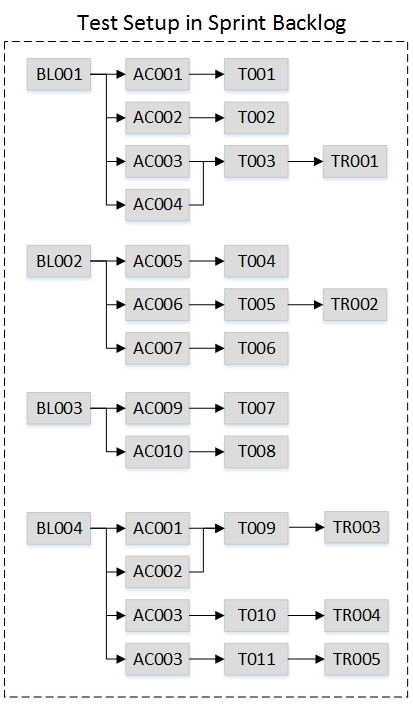
\includegraphics[width=0.55\textwidth]{VAPIQ-PICTURES/testdocbild2}
        \caption{Test Process for Sprint Backlog}
        \label{fig:testsetup2}
\end{figure}
\noindent
Fig. \ref{fig:testsetup2} shows only an example of how we will test Sprint Backlogs. This figure is not related to any already performed tests.\\
\newpage